\documentclass[tikz,border=12pt]{standalone}
\usepackage[T1]{fontenc}
\usepackage{mathpazo}
\usepackage{amsmath,amssymb}
\usetikzlibrary{arrows.meta, calc}

\definecolor{stblue}{HTML}{7B97AD}
\definecolor{rwgold}{HTML}{B8995E}
\definecolor{sage}{HTML}{7A9A7E}
\definecolor{dkbrown}{HTML}{3D3530}
\definecolor{wmgray}{HTML}{7B7067}
\definecolor{cream}{HTML}{F9F6F0}
\definecolor{border}{HTML}{D4C9B8}
\definecolor{terracotta}{HTML}{C47A6A}
\definecolor{lavender}{HTML}{907EA0}

\begin{document}
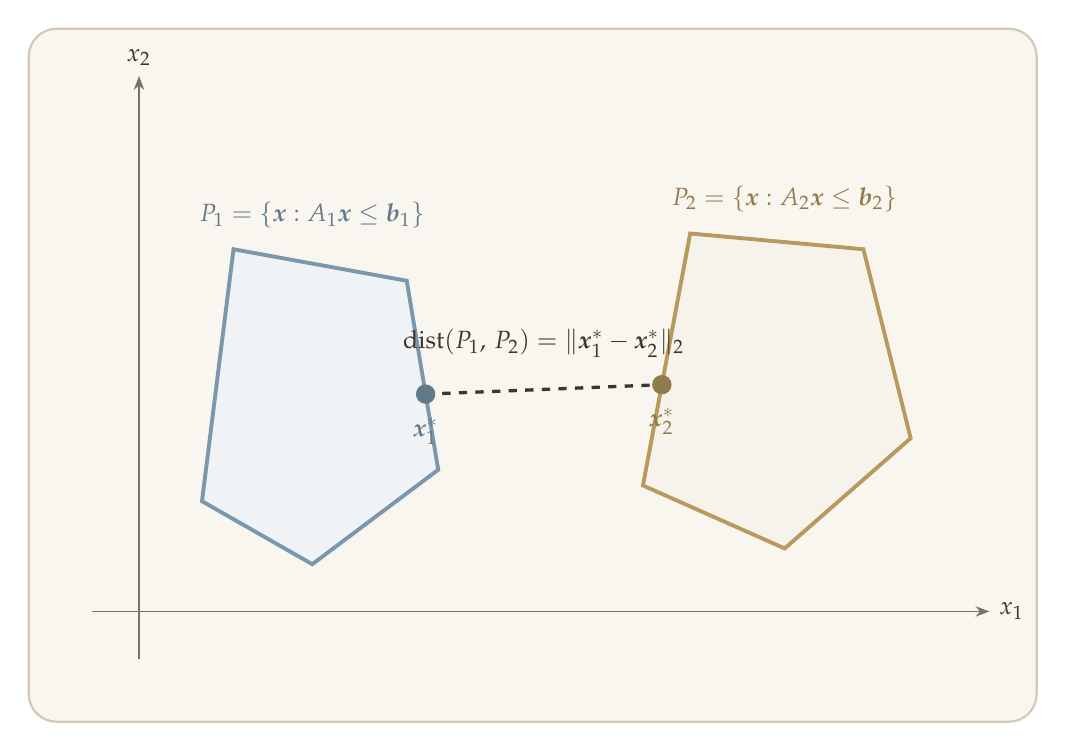
\begin{tikzpicture}[
  >={Stealth[length=3.5mm, width=2.5mm]},
  axis/.style={-{Stealth[length=5pt]}, wmgray, line width=0.6pt},
  lbl/.style={dkbrown, font=\small},
]

% ══════════════════════════════════════════════════════
% Background
% ══════════════════════════════════════════════════════
\fill[cream, rounded corners=10pt] (-1.4,-1.4) rectangle (11.4,7.4);
\draw[border, line width=0.8pt, rounded corners=10pt]
  (-1.4,-1.4) rectangle (11.4,7.4);

% ══════════════════════════════════════════════════════
% Axes
% ══════════════════════════════════════════════════════
\draw[axis] (-0.6,0) -- (10.8,0) node[right, lbl] {$x_1$};
\draw[axis] (0,-0.6) -- (0,6.8) node[above, lbl] {$x_2$};

% ══════════════════════════════════════════════════════
% Polyhedron P1 (left, blue) — 5 vertices
% ══════════════════════════════════════════════════════
\coordinate (P1a) at (0.8, 1.4);
\coordinate (P1b) at (2.2, 0.6);
\coordinate (P1c) at (3.8, 1.8);
\coordinate (P1d) at (3.4, 4.2);
\coordinate (P1e) at (1.2, 4.6);

\fill[stblue!12] (P1a) -- (P1b) -- (P1c) -- (P1d) -- (P1e) -- cycle;
\draw[stblue, line width=1.4pt]
  (P1a) -- (P1b) -- (P1c) -- (P1d) -- (P1e) -- cycle;

% ══════════════════════════════════════════════════════
% Polyhedron P2 (right, gold) — 5 vertices
% ══════════════════════════════════════════════════════
\coordinate (P2a) at (6.4, 1.6);
\coordinate (P2b) at (8.2, 0.8);
\coordinate (P2c) at (9.8, 2.2);
\coordinate (P2d) at (9.2, 4.6);
\coordinate (P2e) at (7.0, 4.8);

\fill[rwgold!12] (P2a) -- (P2b) -- (P2c) -- (P2d) -- (P2e) -- cycle;
\draw[rwgold, line width=1.4pt]
  (P2a) -- (P2b) -- (P2c) -- (P2d) -- (P2e) -- cycle;

% ══════════════════════════════════════════════════════
% Closest points and distance line
% ══════════════════════════════════════════════════════
% x1* on the right edge of P1 (on edge P1c--P1d, ~40% from P1c)
\coordinate (x1star) at (3.64, 2.76);
% x2* on the left edge of P2 (on edge P2e--P2a, ~60% from P2e)
\coordinate (x2star) at (6.64, 2.88);

% Dashed distance line
\draw[dkbrown, dashed, line width=1.2pt] (x1star) -- (x2star);

% Closest point dots
\fill[stblue!80!black] (x1star) circle (3.5pt);
\fill[rwgold!80!black] (x2star) circle (3.5pt);

% Closest point labels — below the dashed line
\node[stblue!80!black, font=\small, anchor=north, yshift=-5pt]
  at (x1star) {$\boldsymbol{x}_1^*$};
\node[rwgold!80!black, font=\small, anchor=north, yshift=-5pt]
  at (x2star) {$\boldsymbol{x}_2^*$};

% ══════════════════════════════════════════════════════
% Distance label — centered above the dashed line
% ══════════════════════════════════════════════════════
\node[dkbrown, font=\small, anchor=south, yshift=8pt]
  at ($(x1star)!0.5!(x2star)$)
  {$\mathrm{dist}(P_1,\, P_2) = \|\boldsymbol{x}_1^* - \boldsymbol{x}_2^*\|_2$};

% ══════════════════════════════════════════════════════
% Polyhedron labels — sitting just above each polygon
% ══════════════════════════════════════════════════════
\node[stblue!80!black, font=\small, anchor=south, inner sep=2pt]
  at (2.2, 4.8)
  {$P_1 = \{\boldsymbol{x} : A_1 \boldsymbol{x} \leq \boldsymbol{b}_1\}$};

\node[rwgold!80!black, font=\small, anchor=south, inner sep=2pt]
  at (8.2, 5.0)
  {$P_2 = \{\boldsymbol{x} : A_2 \boldsymbol{x} \leq \boldsymbol{b}_2\}$};

\end{tikzpicture}
\end{document}
